%
%  MP_talk.tex
%
%  Created by Steven Harms (HOME) on 2011-07-26.
%  Copyright (c) 2011 Steven G. Harms. All rights reserved.
%
\documentclass[slidestop,compress,mathserif]{beamer}
% \documentclass[slidestop,compress,mathserif, slidesonly]{beamer}
% Toggle between 'notes' and no notes to display or undisplay notes pages

% \usepackage[bars]{beamerthemetree}
\usetheme{Warsaw}
\usecolortheme{whale}

% Use utf-8 encoding for foreign characters
\usepackage[utf8]{inputenc}

% Surround parts of graphics with box
\usepackage{boxedminipage}

% Package for including code in the document
\usepackage{listings}

% This is now the recommended way for checking for PDFLaTeX:
\usepackage{ifpdf}

% Support for handouts
\usepackage{pgfpages}
% \pgfpagesuselayout{4 on 1}[a4paper,border shrink=5mm]

% Include support for strikethrough etc.
%\usepackage{ulem}

\ifx\pdftexversion\undefined
\usepackage[dvips]{graphicx}
\else
\usepackage{graphicx}
\DeclareGraphicsRule{*}{mps}{*}{}
\fi
\title{Practical Metaprogramming:  Modeling Thought}
\author{ Steven G. Harms }

\date{2011-09-30}

\begin{document}

\ifpdf
\DeclareGraphicsExtensions{.pdf, .jpg, .tif}
\else
\DeclareGraphicsExtensions{.eps, .jpg}
\fi


\section{Introduction} % (fold)
\label{sec:introduction}

\begin{frame}
	\maketitle
\end{frame}

\subsection{Administration}
\begin{frame}
	\frametitle{Contact Me!}
	\begin{center}
		Steven G. Harms \\
		\vskip 1.25cm
		Physically:  San Francisco, CA\\
		Email:  \texttt{rubyconfXI@sgharms.oib.com} \\
		Twitter / GitHub:  \texttt{sgharms} \\
		G+
	\end{center}
\end{frame}
\note{
Good afternoon, I want to welcome you all to Rubyconf XI back here in The Big Easy!
}

\begin{frame}
	\frametitle{Nawlins}
	\begin{center}
		
\includegraphics[scale=0.50]{img/sazerac.jpg}
		\vskip 0.5cm
		\emph{Be sure to visit the Roosevelt}
	\end{center}
\end{frame}
\note{
It's great to be back here in NO. I spent the early years of my childhood a
little north of here in Slidell. While I spent the rest of my years in Texas,
New Orleans is a wonderful city, with a great character and I'm so glad to
be back here.
}


\subsection{Practicality}

\begin{frame}
	\frametitle{What We'll Cover}
	\begin{center}
		Practical Metaprogramming
	\end{center}
\end{frame}

\begin{frame}
	\frametitle{\textbf{Im}-practical Metaprogramming}
	\pause
	\begin{center}
		
\includegraphics[scale=0.3]{img/rubyrogues.png}
	\end{center}
	\vskip 0.25cm
	Episode 012:  Metaprogramming
	\vskip 0.25cm
	\begin{itemize}
		\pause
		\item 10 minutes into attempting to define ``metaprogramming'' they had covered{\ldots}
		\begin{itemize}
			\item Lisp
			\pause
			\item Marshaling code, closures, state 
			\pause
			\item Code as data?  AST's versus bytecode?
			\pause
			\item Code generation versus runtime behavior changes
		\end{itemize}
	\end{itemize}
\end{frame}

\begin{frame}
	\frametitle{Huh?}
	\begin{center}
		
\includegraphics[scale=0.5]{img/chan.png}
	\end{center}
\end{frame}

\begin{frame}
	\frametitle{\textbf{Im}-practical Metaprogramming:  Metaprogramming \textbf{un}-defined}
	Working definitions proposed:
	\begin{itemize}
		\item ``Code that writes code''
		\pause
		\item ``API for dynamic programming within the Ruby language''
		\pause
		\item ``Programming other peoples' programs''
		\pause
		\item ``Bowkett:  There's no such thing as MP, there is just programming''
		\pause
		\item ``Things that treat code as data''
		\pause
		\item ``Anything that would blow the mind of a Java programmer.''
	\end{itemize}
\end{frame}
\note{
	\begin{itemize}
		\item All of these are true
		\item Unfair to pick on misuse in the next segment
	\end{itemize}
}

\begin{frame}
	\frametitle{Practical Metaprogramming}
	\begin{itemize}
		\pause
		\item Written by a Ruby Average Joe{\texttrademark}, Steven Harms, not Ruby-legend
		\pause
		\item Focuses on relatable experiences, not theory
		\pause
		\item Builds from basic Ruby
	\end{itemize}
\end{frame}

\subsection{Benefit To You} % (fold)
\label{sub:benefits}

\begin{frame}
	\frametitle{Why You Need To Learn This:  Precedent}
	\begin{enumerate}
		\item Virtually all core libraries make use of MP
		\pause
		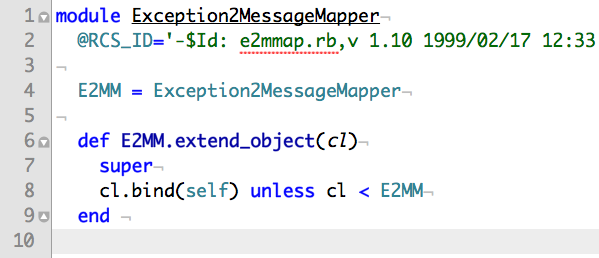
\includegraphics[scale=0.45, width=0.89\textwidth]{img/e2mmap.png}
		\pause
		\item Rails uses MP all over the place
	\end{enumerate}
\end{frame}

\begin{frame}
	\frametitle{Why You Need To Learn This:  Your Future}
	\begin{enumerate}
		\item Save yourself a lot of typing
		\pause
		\item Reflect the interior world of your problem domain (including ambiguity!) in your application code
		\pause
		\item Pleasant surprises
	\end{enumerate}
\end{frame}
\note{I believe you will start to see some of these benefits if I am able to attain some of the following goals in this presentation.}

\subsection{Goals} % (fold)
\label{sub:goals}

\begin{frame}
	\frametitle{Goals}
	\begin{enumerate}
		\item Dispel FUD around metaprogramming: you should metaprogram \textbf{boldly} -- \emph{I want you to feel awesome!}
		\pause
		\begin{itemize}
			\item Demonstrate that metaprogramming is ``just programming''
			\pause
			\item Describe four ``tiers'' of metaprogramming spells so you know how to ``level up''
		\end{itemize}
		\pause
		\item Let the ancestor chain guide us (\emph{``Gray's Mandate''})
		\pause
		\item Show a real-world example of the benefits of MP
	\end{enumerate}
\end{frame}

\begin{frame}
	\frametitle{Gray's Mandate}
	\begin{center}
		\emph{Ruby's method call system is really important{\ldots}and you have to get your
head around it at some point about how it does these lookups{\ldots}method call
system is a straight line with stops along the way…once you get the hang of
it{\ldots}you realize you can put a module at any point on that line.}
	-- James Edward Gray II (\texttt{@JEGII}), Ruby Rogues ep. 012, $\approx$ 23m
	\end{center}
\end{frame}

% subsection goals (end)

\subsection{Audience} % (fold)
\label{sub:audience}
\begin{frame}
	\frametitle{Audience}
	Beginner / Intermediate Rubyists will benefit from the first part of this talk.
	\vskip 2.0cm
	Intermediate/Advanced Rubyists will benefit from the ``metaprogramming in the wild'' demonstration that uses my library \texttt{LatinVerb}
\end{frame}
\note{
That's the lay of the land for this talk. If you're thinking this talk might
not be for you, then you're welcome to hop over to the other tracks.
}
% subsection audience (end)

\begin{frame}
	\frametitle{Intermission}
	\begin{center}
		\texttt{INTERMISSION}
	\end{center}
\end{frame}

\begin{frame}
	\frametitle{Socially Awkward Penguin}
	\begin{center}
		
\includegraphics[scale=0.3]{img/sap.png}
	\end{center}
\end{frame}
\note{
Whew, I'm glad we only lost those few.
}

\begin{frame}
	\frametitle{End Slide if Everyone Leaves}
	\begin{center}
		
\includegraphics[scale=0.15]{img/forever_alone.png}
		\vskip 0.5cm
		\emph{Forever Alone{\ldots}}
	\end{center}
\end{frame}


\section{Practical MP} % (fold)
\label{sub:practical_metaprogramming}

\subsection{Early Exposure} % (fold)
\label{sub:early_exposure}

\begin{frame}
	\frametitle{``Practical Metaprogramming:  First Contact''}
	\begin{center}
		
\includegraphics[scale=0.55]{img/first_contact.jpg} \\
	\end{center}
	\emph{\ldots and is it to be called an ``eigenclass'' or a ``singleton class,'' ma'am?}
\end{frame}
\note{
	\begin{itemize}
		\item 
	\end{itemize}
}

\begin{frame}
	\frametitle{So, seriously, what \textbf{is} metaprogramming?}
	\begin{center}
		\pause
		``Writing code that re-directs passed messages at runtime \\ \textbf{or} \\
that provides or alters the structures that do said passing.''
		\pause
		\emph{\\ --Steven Harms}
	\end{center}
\end{frame}
\note{}

\begin{frame}
	\frametitle{But wait{\ldots}isn't that just \emph{regular} programming?}
	\begin{center}
		Yes.  Exactly.  Ergo:  ``There is no metaprogramming -- just programming''
		\pause
		\vskip 0.25cm
		\emph{Let's see it in action}
	\end{center}
\end{frame}

\begin{frame}
	\frametitle{Start simply}
		\begin{center}
			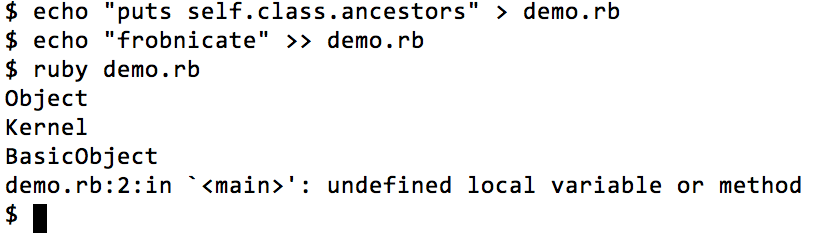
\includegraphics[scale=0.35]{img/undefined_method_chain.png}
		\end{center}
\end{frame}

\begin{frame}
	\frametitle{Why did this fail?}
	\pause
	\begin{center}
		\emph{Because a message was passed that Ruby did not know about}
		\vskip 0.75cm
		\pause
		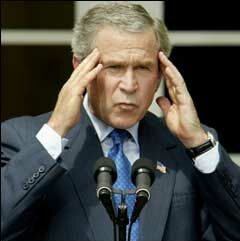
\includegraphics[scale=0.80]{img/duh.jpg}		
	\end{center}
\end{frame}

\begin{frame}
	\frametitle{``How can we re-direct this message?''}
	\pause
	\begin{center}
		\texttt{\textbf{def}} \\
		\vskip 0.5cm
		\pause		
		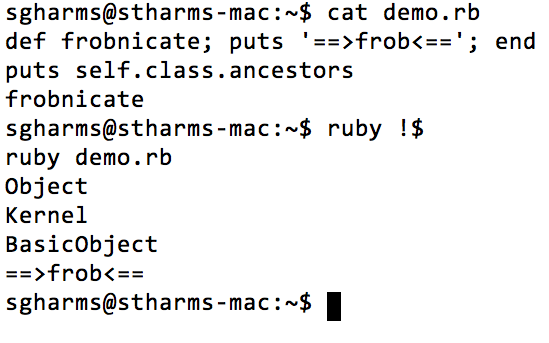
\includegraphics[scale=0.45]{img/def_as_mp.png}		
	\end{center}
\end{frame}
\note{
Here we have put the def into the default ``main'' object of the Ruby.  

Now we're programmers, we like to keep things nice and neat.  So we might want to try
to put our re-director into something -- like a class.
}

\begin{frame}
	\frametitle{Put the \texttt{defs} in a class}
	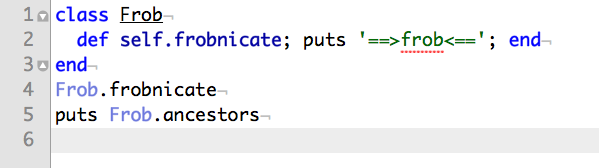
\includegraphics[scale=0.45]{img/frob_classmethod.png} \\
	\vskip 0.25cm
	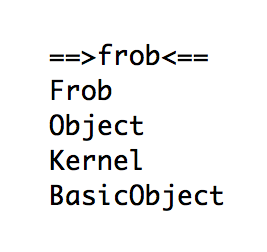
\includegraphics[scale=0.45]{img/frob_classmethod_output.png}		
\end{frame}

\begin{frame}
	\frametitle{Put the \texttt{def}s in a module}
	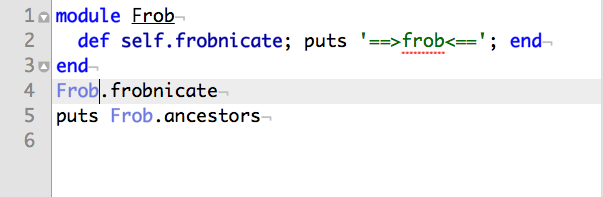
\includegraphics[scale=0.45]{img/frob_module.png} \\
	\vskip 0.25cm
	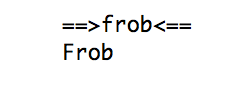
\includegraphics[scale=0.45]{img/frob_module_output.png}		
\end{frame}

\begin{frame}
	\frametitle{Put the \texttt{def}s in the module into the class (\emph{mixin})}
	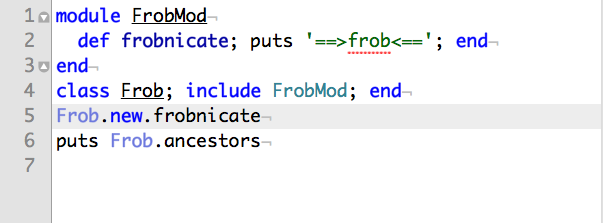
\includegraphics[scale=0.45,scaleY=0.8]{img/frob_mixin.png} \\
	\vskip 0.25cm
	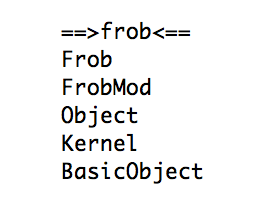
\includegraphics[scale=0.45]{img/frob_mixin_output.png}		
\end{frame}

\begin{frame}
	\frametitle{Put the \texttt{def}s in the module\textbf{s} into the class (\emph{mixin})}
	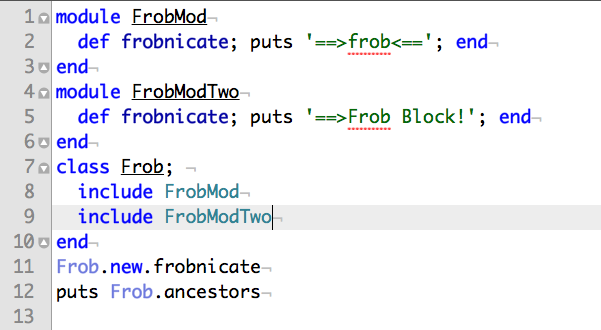
\includegraphics[scale=0.45,height=4cm]{img/frob_double_mod.png} \\
	\vskip 0.20cm
	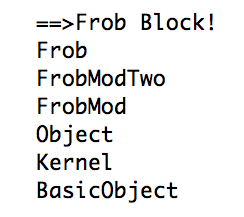
\includegraphics[scale=0.45]{img/frob_double_mod_output.png}		
\end{frame}

\begin{frame}
	\frametitle{Put the \texttt{def}s in the modules based on random}
	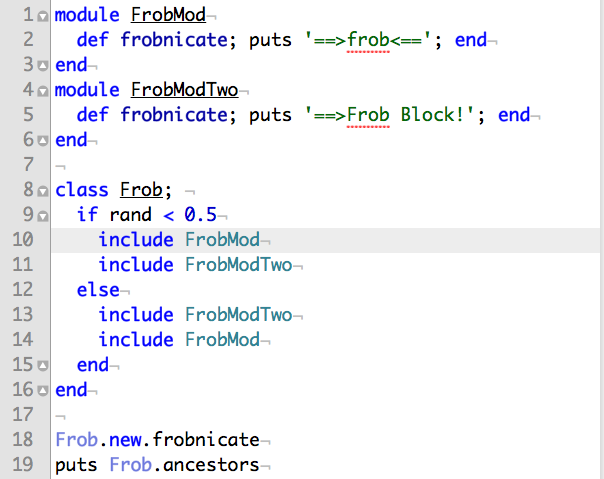
\includegraphics[scale=0.45]{img/frob_random.png} \\
\end{frame}

\begin{frame}
	\frametitle{Sometimes Ancestors Look Like\ldots}
		\path{Frob}\\
		\path{FrobModTwo}\\
		\path{FrobMod}\\
		\path{Object}\\
		\path{Kernel}\\
		\path{BasicObject}\\
\end{frame}

\begin{frame}
	\frametitle{And Sometimes Look Like\ldots}
		\path{Frob}\\
		\path{FrobMod}\\
		\path{FrobModTwo}\\
		\path{Object}\\
		\path{Kernel}\\
		\path{BasicObject}\\
\end{frame}

\begin{frame}
	\frametitle{Quod Erat Demonstrandum{\ldots}}
	With:
	\begin{itemize}
		\item Ancestor chain
		\item Modules and Classes
	\end{itemize}
	\vskip 0.25cm
	Catching, intercepting, and re-routing messages based on conditions (e.g.
\texttt{rand}) occurs. 
\vskip 0.25cm 
We ``wrote code that re-directed passed messages at
runtime or that provided or altered the structures that do said processing.''

\end{frame}

\begin{frame}
	\frametitle{We were metaprogramming!}
	\begin{itemize}
		\item We were metaprogramming (by my definition)
		\pause
		\item We used only techniques from Ruby basics tutorials (e.g. \texttt{def},
\texttt{module}, \texttt{class}) but reacted and re-directed based on runtime
logic ( \texttt{$>$rand})
		\pause
		\item Therefore:  Either metaprogramming is much easier than we thought, OR
		\pause
		\item The difference between ``programming'' and ``metaprogramming'' is unimportant
	\end{itemize}
\end{frame}

\begin{frame}
	\frametitle{That Said\ldots}
	\begin{itemize}
		\item It is convenient to refer to metaprogramming as a \emph{style} of programming
		\item When the language has a clear function to do X, don't write a MP re-implementation without good reason
	\end{itemize}
\end{frame}
\note{Now that we see that we've all been quote-metaprogramming since the beginning
of our Ruby careers. Let's dispel some of the fear about the quote-advanced
metaprogramming techniques. I hope to offer 4-part sectioning of common MP
spells, or idioms that will help you measure and evaluate your skill with this
subset of the Ruby language.}

\begin{frame}
	\frametitle{Momentary Aside: Terminology}
	``Spells'' and their names derive from \underline{Metaprogramming Ruby} by Paolo ``Nusco'' Perrotta:
	\vskip 0.5cm
	\begin{center}
		\underline{http://ducktypo.blogspot.com/2010/08/} \\
		\underline{metaprogramming-spell-book.html}
	\end{center}
\end{frame}
\note{
	\begin{itemize}
		\item Using the terminology provided by Perrotta
		\item The names are good
		\item As a community needs a common lexicon for reference
		\item There are about 30 of these ``spells,'' as Paolo calls them.
	\end{itemize}
}

\begin{frame}
	\frametitle{Metaprogramming Pre-Requisites}
	\begin{itemize}
		\item Basic Method Manipulation
		\item Basic Class Definition
		\item Basic Module Definition
		\item The Mix-In
	\end{itemize}
\end{frame}
\note{We just covered these}

\begin{frame}
	\frametitle{Tier 1 Metaprogramming: \emph{Advanced Message Redirection}}
	\begin{itemize}
		\item Open Class
			\begin{itemize}
				\item Kernel Method
				\item Monkeypatch
			\end{itemize}
		\item \texttt{attr\_*} methods
		\item alias :new :old
	\end{itemize}
	\vskip 0.5cm
\end{frame}


\begin{frame}
	\frametitle{Tier 1 Metaprogramming:  Open Classes}
		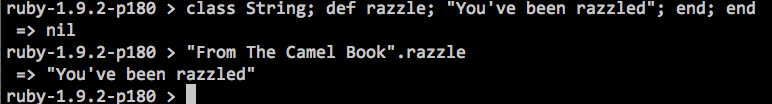
\includegraphics[scale=0.42]{img/open_class.png}
\end{frame}
\note{
	\begin{itemize}
		\item Starts here
		\item You can add methods to an existing \textbf{core} class
		\item ``Open Class'' spell
	\end{itemize}
}

\begin{frame}
	\frametitle{Tier 1 Metaprogramming:  Kernel Method}
		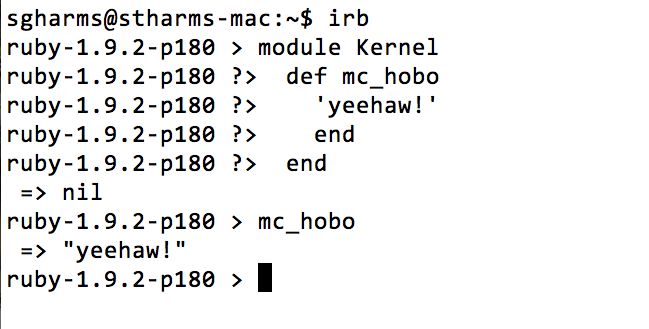
\includegraphics[scale=0.55]{img/kernel_method.png}
\end{frame}
\note{
At this point we're starting to feel some power here. We now see that we can
create methods that behave as if they were core builtins to the language.
}

\begin{frame}
	\frametitle{Tier 1 Metaprogramming:  Dynamic Getter / Setter Generation}
	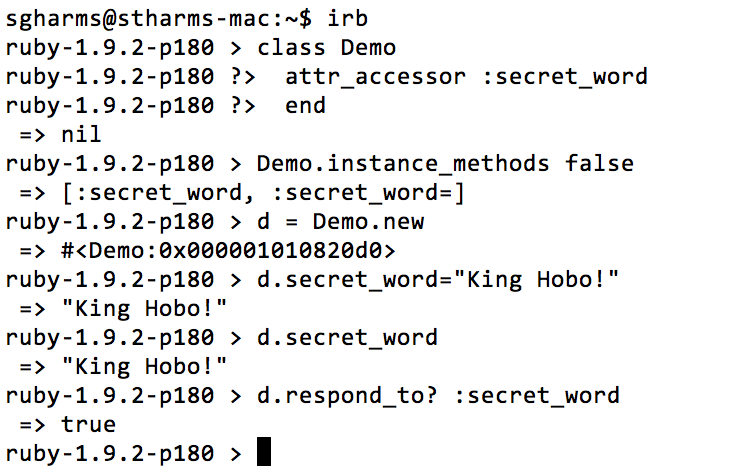
\includegraphics[scale=0.45]{img/attr_demo_1.png}
\end{frame}


\begin{frame}
	\frametitle{Tier 1 Metaprogramming: Singleton Method}
		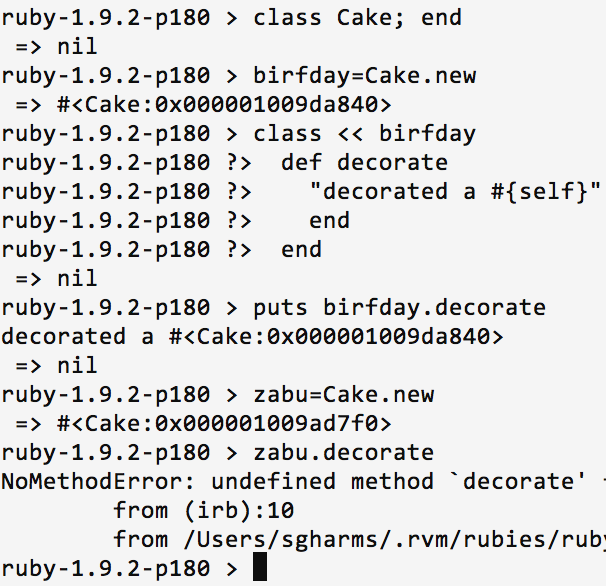
\includegraphics[scale=0.35]{img/singleton_method.png}
\end{frame}
\note{
	\begin{itemize}
		\item Jerks tears from Java programmers
		\item This is undoubtedly the one that makes the pro-Java camp weep.
		\item In compiled languages the definition of a class represents a static contract between the developer and the compiler.
		\item A class is an expression of that contract.
		\item In Ruby, a class is really a namespace expression.
		\item Simple truth that is easy to hear, but hard to \emph{understand}.
		\item \textbf{THIS IS AWESOME}
	\end{itemize}
}

\subsection{Danger Zone} % (fold)
\label{sub:danger_zone}

\begin{frame}
		\frametitle{AWESOMENESS}
		\begin{center}
			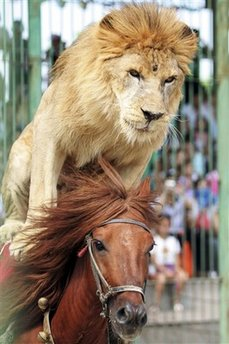
\includegraphics[scale=0.45]{img/lion_horse.jpg} \\
			\emph{-- Credit Unknown}
		\end{center}
\end{frame}
\note{It might not be the most awesome thing ever, which is, of course, a lion
riding a horse, but it's still pretty good.}

\begin{frame}
	\frametitle{{\ldots}Or Madness?}
	Incautiously used, these lead to the dangers of MP:
	\begin{itemize}
		\item Opaqueness
		\item Unpredictability
		\item Unsupportability
	\end{itemize}
\end{frame}
\note{This quickly becomes side-effect soup.  So much so that you get elements of doubt.}

\begin{frame}
	\frametitle{Thesis:  F.U.D.}
		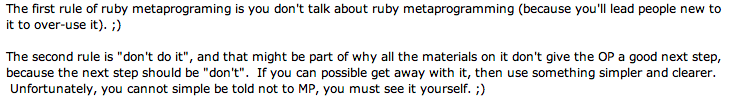
\includegraphics[width=0.98\textwidth, height=0.25\textheight]{img/tim_hates_mp.png}
		\vskip 0.5cm
		\emph{--Tim Connor:  SF Ruby Mailing List}
\end{frame}
\note{
	I had a mail from Tim and his personal views aren't as strong as this, but
he's definitely urging caution over MP's over-use.
}

\begin{frame}
	\frametitle{Antithesis:  anti-F.U.D.}
	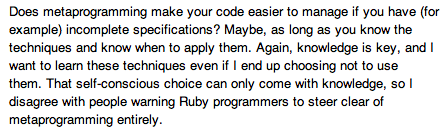
\includegraphics[width=0.98\textwidth, height=0.45\textheight]{img/paolo_anti_fud.png}
	\vskip 0.5cm
	\emph{--Paolo Perrotta, author of Metaprogramming Ruby, in e-mail to Steven Harms}
\end{frame}
\note{
\begin{itemize}
	\item Leaves quite a bit to chance
	\item This attitude implies that we think the material is optional or unimportant.
	\item It is not
\end{itemize}
}

\subsubsection{Teenagers} % (fold)
\label{ssub:teenagers}

\begin{frame}
	\frametitle{Teens:  Foolishness}
	\begin{center}
		
\includegraphics[scale=0.1]{img/license.jpg}
	\end{center}
	
\end{frame}
\note{All the power and free will of an adult, but not a whole lot of judgment, and poor impulse control.}

\begin{frame}
	\frametitle{Teens:  Brilliance}
	\begin{center}
		
\includegraphics[scale=0.25]{img/daniel.jpg}	
	\end{center}
	
\end{frame}

\begin{frame}
	\frametitle{Synthesis:  Good Parenting, or Alloparenting}
	\begin{center}
		\emph{``{\ldots}if root's strong, tree survive''} \\
		-- Mr. Miyagi
	\end{center}
	\begin{itemize}
		\item Singleton Module (``Eigenclass'')
		\item \texttt{Module\#ancestors}
	\end{itemize}
\end{frame}
\note{You all have a good root, but be careful with these!  You'll paint yourself into a corner or two, but keep a git branch or two handy.}

% subsubsection teenagers (end)

\begin{frame}
	\frametitle{How Will I Know?}
	\begin{center}
		
\includegraphics[scale=0.10]{img/whitney.jpg}
	\end{center}
\end{frame}
\note{
  \emph{Quickly}: Turn the \underline{benefits} just described into \underline{conditions}.
}

\begin{frame}
	\frametitle{Explain this: Why are these methods identical structurally?}
	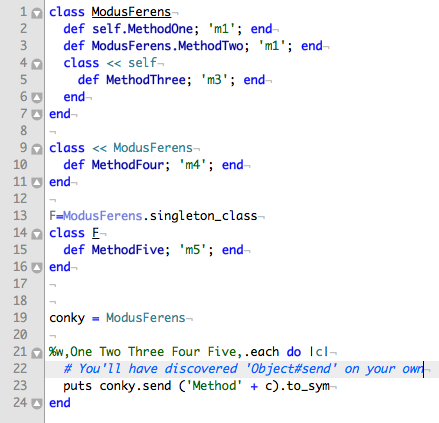
\includegraphics[scale=0.50]{img/challenge.png}
\end{frame}

\subsection{Tier 2 MP} % (fold)
\label{sub:tier_2_metaprogramming_idioms}

\subsubsection{Idioms} % (fold)
\label{ssub:idioms}

\begin{frame}
	\frametitle{Tier 2 Metaprogramming Idioms}
	\begin{itemize}
		\item Generally, methods for the interception and interpretation of passed messages \emph{as handled by you!}
		\item Hybrids involving earlier techniques
	\end{itemize}
	\pause
	\begin{itemize}
		\item Dynamic Dispatch:  \texttt{Object\#send}
		\pause
		\item Method Missing:  use \texttt{method\_missing(sym,\*args)} 
		\pause
		\item Ghost Method:  call methods on a BasicObject to trigger \texttt{method\_missing}
		\pause
		\item Around Alias:  Monkeypatch a method call and keep a reference to the original
	\end{itemize}
\end{frame}
\note{
I will not dwell on these because they are rather complicated \textbf{and} are discoverable via Paolo's book or his site.  Third,
Also, I will be demonstrating them shortly.
}
% subsubsection idioms (end)
% subsection tier_2_metaprogramming_idioms (end)

\subsection{Tier 3 MP} % (fold)
\label{sub:tier_3_metaprogramming}

\begin{frame}
	\frametitle{Tier 3 Metaprogramming}
	\begin{itemize}
		\item Dynamic Generation and Inclusion of Modules
		\begin{itemize}
			\item Namespace:  Dynamically generate 
			\item Class Extension:  Dynamically include
		\end{itemize}
		\item No-holds-barred manipulation of classes and instances
		\begin{itemize}
			\item class\_eval 
			\item instance\_eval 
		\end{itemize}
	\end{itemize}
\end{frame}

\begin{frame}
	\frametitle{Word from Mom and Dad}
	\begin{center}
		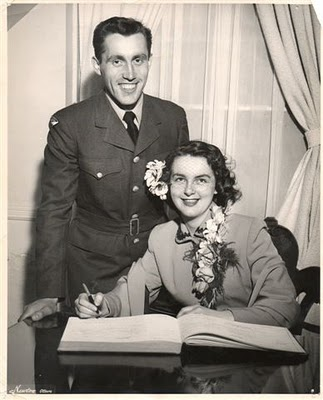
\includegraphics[scale=0.35]{img/MomDadMarried50s.jpeg}
	\end{center}
	\pause
	\begin{itemize}
		\item Most advanced techniques are fancy syntax for the basic techniques
		\pause
		\item Uncle Ben's Axiom:  With great power comes great responsibility
	\end{itemize}	
\end{frame}
% subsection tier_3_metaprogramming (end)

\section{LatinVerb Demo} % (fold)
\label{sub:_modeling_thought_in_latinverb}

\begin{frame}
	\frametitle{Demo}
	\begin{center}
		\texttt{LatinVerb}
	\end{center}
\end{frame}

\begin{frame}
	\frametitle{Or as Aaron Patterson once said:}
	\begin{center}
		``Do something worthless of questionable value.'' \\ -- \emph{Aaron Patterson}
	\end{center}
\end{frame}
\note{
So, let's talk about how I went about modeling this problem.  Here's a specification.
}

\begin{frame}
	\frametitle{Specification}
	\begin{itemize}
		\item Given the \underline{four principle parts}:  ``am\={o}, am\={a}re, am\={a}v\={\i}, amatum''
		\pause
		\item Respond with a unique value (``conjugation''), \emph{am\={o}}, to a call with the parameters: \\
		``active voice indicative mood present tense first person singular number'' (Fully-Qualified)
		\pause
		\item Flexibly respond to calls that lack some specification datum e.g. leave out the ``number'' parameter, receive with less-granular return values\\
          e.g. ``active voice indicative mood present tense'' (3 aspects provided, 6 results)
	\end{itemize}
\end{frame}

\begin{frame}
	\frametitle{Tabular View}
	\begin{center}
		\begin{tabular}{|c|c|c|}
			\hline
			  & Singular Number &  Plural Number\\
			\hline
			First Person  & laud\={o}  & laud\={a}mus\\
			Second Person & laud\={a}s & laudatis \\
			Third Person  & laudat     & laudant \\
			\hline
		\end{tabular}
	\end{center}
\end{frame}

\begin{frame}
	\frametitle{Model it in Ruby!}
	\begin{center}
		
\includegraphics[scale=0.45]{img/brosh_all.png}
		\vskip 0.5cm
		\emph{Credit:  Allie Brosh}
	\end{center}
\end{frame}

\begin{frame}
	\frametitle{Painful Combinations}
	\begin{itemize}
		\item 6 results means 6 methods to be defined \emph{per tense}
		\pause
		\item \ldots $\times$ 6 tenses (present/imperfect/future/perfect/past-perfect/future-perfect)
		\pause
		\item \ldots $\times$ 2 voices (active/present)
		\pause
		\item \ldots \emph{and then there's another mood with 4 tenses of its own!}
		\pause
		\item Each regular Latin verb has $\approx$  160 unique vectors
		\pause
		\item There are 5 standard paradigms
		\pause
		\item \ldots and at least $1,000$ verbs
		\pause
		\item Possibly thousands of methods or decision flows in a language with poor MP
	\end{itemize}
\end{frame}

\begin{frame}
	\frametitle{Metaprogramming Makes a Saving Throw!}
	\begin{center}
		MP our way out of the pain
		\vskip 1.0cm
		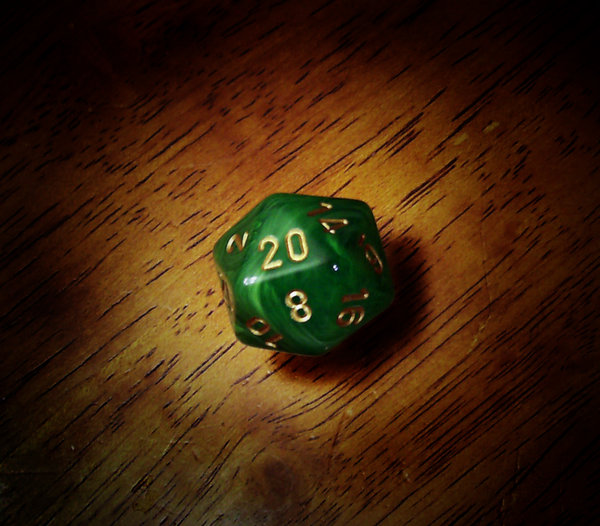
\includegraphics[scale=0.25]{img/natural_20.jpg} \\
		\tiny
		\emph{Credit: Marco26 on DeviantArt}
		\normalsize
	\end{center}
\end{frame}

\begin{frame}
	\frametitle{Stuff the logic in the TenseBlock Class}
	\emph{
		Sub-specify by \underline{person} (1, 2, 3) or \underline{number} or
    cluster by either. \\
		\pause
		{\ldots} and allow terms in method call to be reordered
  }
	\vskip 0.5cm
	\begin{center}
		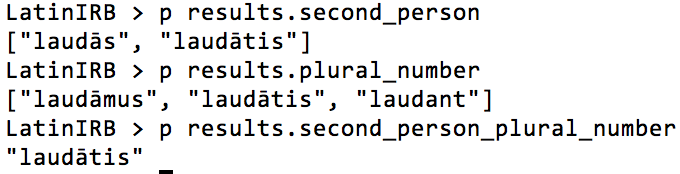
\includegraphics[scale=0.38]{img/conj_subspec.png}
	\end{center}
\end{frame}

\begin{frame}
	\frametitle{\texttt{method\_missing} and dynamic dispatch(\texttt{send})}
	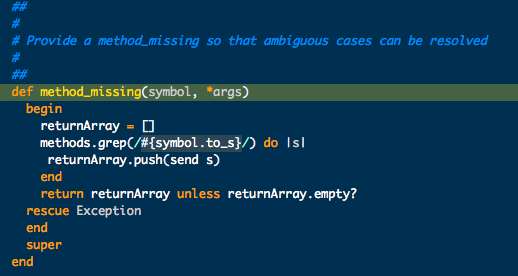
\includegraphics[scale=0.45]{img/tenseblock_mm.png}
\end{frame}

\begin{frame}
	\frametitle{MP Provides:  Massive Laziness Win}
	\begin{itemize}
		\item $\approx$ 48 methods covered; 6 written
		\pause
		\item One response class (\texttt{TenseBlock})
	\end{itemize}
\end{frame}

\begin{frame}
	\frametitle{Table becomes TenseBlock}
	\begin{center}
		\begin{tabular}{|c|c|c|}
			\hline
			  & Singular Number &  Plural Number\\
			\hline
			First Person  & laud\={o}  & laud\={a}mus\\
			Second Person & laud\={a}s & laudatis \\
			Third Person  & laudat     & laudant \\
			\hline
		\end{tabular}
		\vskip 0.5cm
		$=$
		\vskip 0.5cm
		\texttt{TenseBlock}
	\end{center}
\end{frame}

\begin{frame}
	\frametitle{Not Bad}
	
\includegraphics[scale=0.75]{img/not_bad.png}
\end{frame}

\begin{frame}
	\frametitle{Scale it Up!: Dynamic Dispatch in \texttt{method\_missing}}
	\begin{center}
		\emph{Be flexible on all 5 aspects}
	\end{center}
	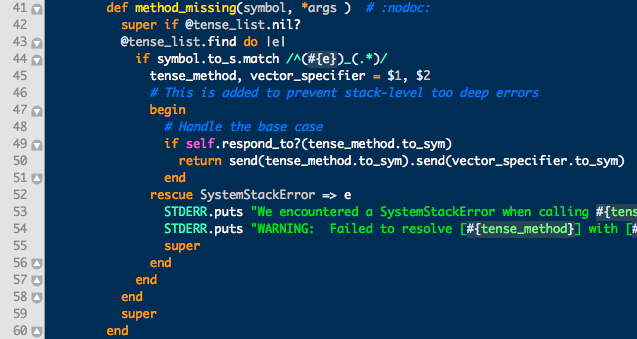
\includegraphics[scale=0.45]{img/lv_mm.png}
\end{frame}
\note{
The same technique that we used with a Tense Block that gave each one several extra methods, I then scaled that shortcut by doubling the dynamic method call.
}

\begin{frame}
	\frametitle{Result:  Super-Massive Laziness Win}
	\begin{itemize}
		\item Covered the thousands of methods predicted
		\pause
		\item \ldots and provided the clustering methods as well as a surprising bonus
	\end{itemize}
	\pause
	\vskip 0.5cm
	\emph{I only wrote 24 methods}
\end{frame}

\begin{frame}
	\frametitle{Result:  Surprises}
	\begin{itemize}
		\item ``Aggregator methods'' per tense emerged
		\item Flexible word order \emph{emerged} that did the right thing
		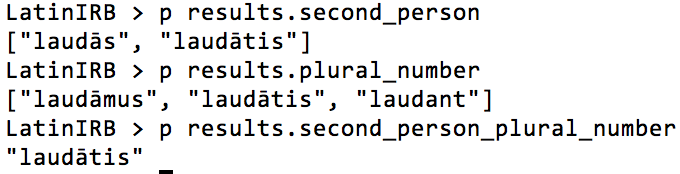
\includegraphics[scale=0.38]{img/conj_subspec.png}
		\pause
		\item Avoided Java-ish paramteterized brain damage
	\end{itemize}
\end{frame}


\begin{frame}
	\frametitle{Java-ish Brain Damage:  Parameterization}
 	\texttt{String calculate\_vector(VerbyType aV, String v, String m, String t, String p, String n)}
	\vskip 0.5cm

	\begin{center}
		\textbf{OR}
	\end{center}

	\vskip 0.5cm
	\texttt{Object[] calculated\_values = \{aV, v, m, t, p, n\};}
	\texttt{String calculate\_vector(calculated\_values)};
	\vskip 0.5cm

	\begin{center}
		\textbf{PREFER}
	\end{center}

	\vskip 0.5cm
	\texttt{@aFirst.active\_voice\_indicative\_mood{\ldots}}
\end{frame}
\note
{A particular reason that I want to highlight this benefit is because
Java/C-style parameterization is not how we think. It is certainly not how
linguists think. Further, the form takes this really nice Objective-C
stylistic that I think is very clear and sexy.
}

\begin{frame}
	\frametitle{Usage of Third-Tier Metaprogramming in LatinVerb}
	\begin{itemize}
		\item DSL:  \emph{See Evan's talk from Lone Star Ruby Conf}
		\item Class Extension a.k.a. Mixin
		\item Module namespace cleanliness
	\end{itemize}
\end{frame}

\begin{frame}
	\frametitle{Listen to your mentors}
	\begin{itemize}
		\item David Brady:  ``Use modules, kids.''
		\item JEG2:  ``Understand your ancestor chain''
		\item Jim Weirich:  ``Polite programmers \texttt{respond\_to?} with true for their metaprogrammed methods''
		\item Corey Haines:  ``Extraction into modules allows you to build super-fast tests! (\emph{GoGaRuCo 2011})''
	\end{itemize}
\end{frame}

\begin{frame}
	\frametitle{Build beautiful module generators}
	\begin{center}
		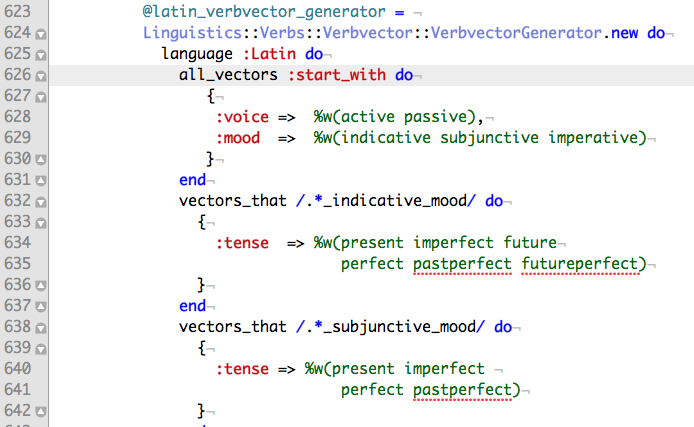
\includegraphics[scale=0.35]{img/ll_dsl.png} \\
		\emph{from \texttt{latinverb.rb}}
	\end{center}	
\end{frame}

\begin{frame}
	\frametitle{Build beautiful module generators}
	\begin{center}
		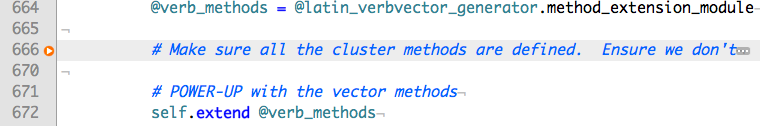
\includegraphics[scale=0.35]{img/ll_mod_inc.png}
	\end{center}	
\end{frame}

\begin{frame}
	\frametitle{\texttt{respond\_to?} and \texttt{ancestors}}
	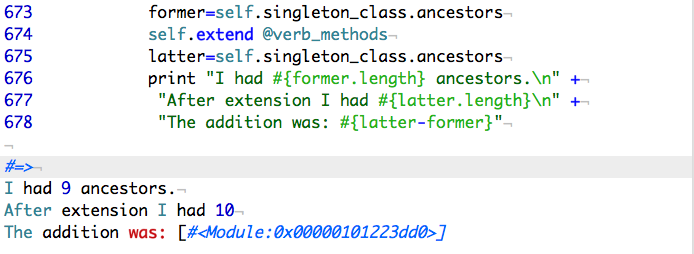
\includegraphics[scale=0.45]{img/method_chain_first.png}
\end{frame}

\begin{frame}
	\frametitle{\texttt{respond\_to?} and \texttt{ancestors}}
	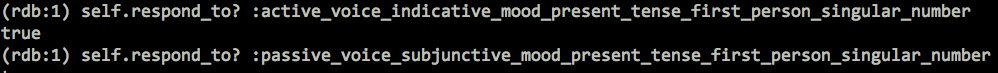
\includegraphics[width=10cm, height=0.75cm]{img/respond_to_well.png}
\end{frame}

\begin{frame}
	\frametitle{Greatest Benefit: Clarity \& Communication}
	\begin{center}
		\emph{``Code that Communicates''}
		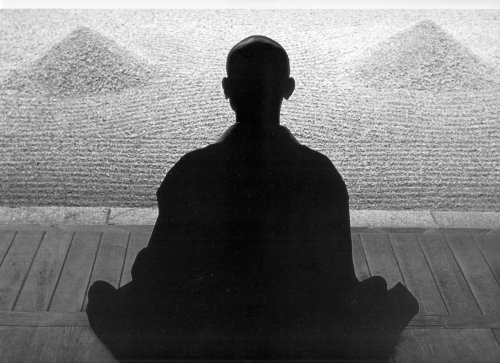
\includegraphics[scale=0.45]{img/Zen04.jpg}
	\end{center}
\end{frame}
\note{Despite quote-metaprogramming getting such a bad rap, it really doesn't
\emph{only} obfuscate -- sometimes it really \emph{helps}!}

\begin{frame}
	\frametitle{Goals Checklist}
	\begin{enumerate}
		\item ``Metaprogram'' \textbf{boldly}!
		\begin{itemize}
			\pause
			\item Metaprogramming is ``just programming'' -- \emph{and you're already better at it than you know!}
			\pause
			\item Study and experiment with the four ``tiers'' of metaprogramming spells
			\pause
			\item Remain humble and continue to listen for guidance
		\end{itemize}
		\pause
		\item Use the ancestor chain as your guide -- \emph{Answer Gray's mandate \textbf{boldly}!}
		\pause
		\item Let MP surprise you, model ambiguity cleanly, and help communicate your domain
		\pause
		\item Thank the Ruby Rogues for taking a bit of a ribbing
	\end{enumerate}
\end{frame}

\section{Supplementary} % (fold)
\label{sec:supplementary}

\begin{frame}
	\frametitle{Supplementary}
	\begin{center}
		Supplementary Information
	\end{center}
\end{frame}

\begin{frame}
	\frametitle{Book}
	\underline{Metaprogramming Ruby} by Paolo Perrotta
\end{frame}

\begin{frame}
	\frametitle{List of Spells}
	\texttt{http://ducktypo.blogspot.com/2010/\\08/metaprogramming-spell-book.html}
\end{frame}

\begin{frame}
	\frametitle{(Meta)programming Politely}
	\texttt{http://confreaks.net/videos/\\374-rubyconf2010-the-polite-programmer-s-guide-to\\-ruby-etiquette}
\end{frame}

\begin{frame}
	\frametitle{Photo Credits}
	\begin{enumerate}
		\footnotesize
		\item ``Zen'' pic:\\ \texttt{http://www.insidesocal.com/tomhoffarth/archives/2011\\
		 /06/shawn-greens-ze.html}
		\normalsize
	\end{enumerate}
\end{frame}

\begin{frame}
	\frametitle{Colophon}
	\LaTeX and the Beamer Slide Toolkit
\end{frame}

\begin{frame}
	\frametitle{SpeakerRate}
	\center{Help Me Get Better!}
	\vskip 1.25cm
	\begin{center}
		\texttt{http://spkr8.com/t/8534}
	\end{center}
\end{frame}

\begin{frame}
	\frametitle{Work with Me / Have Me Teach / Contact Me!}
	\begin{center}
		\LARGE
		Thank You! \\
		\normalsize
		\vskip 0.75cm
		Steven G. Harms \\
		\vskip 0.75cm
		Physically:  San Francisco, CA\\
		Email:  \texttt{rubyconfXI@sgharms.oib.com} \\
		Twitter / GitHub:  \texttt{sgharms} \\
		G+
		\vskip 1.0cm
				\texttt{http://spkr8.com/t/8534}
		\vskip .80cm
		Questions?
	\end{center}
\end{frame}

\end{document}

